\chapter{A multi-view modeling framework\label{chapter:framework}}

This chapter installs the background necessary for understanding subsequent chapters of this thesis. 

\newcommand{\artifact}[1]{\texttt{#1}}

\section{Running example: A toy train system}

We use a simple train system fragment as running example for illustrating concepts and techniques throughout this thesis. The system is composed of an automated train controller, actuators for doors and the engine as well as the latter themselves, a sensor of the train speed and a passenger. Via the actuators, the controller typically controls operations like starting or stopping the train, opening or closing the doors, and so on. A safety goal requires train doors to remain closed while the train is moving. If the train is not moving and the passenger presses the alarm button, the controller must open the doors immediately. If the train is moving and the passenger presses the alarm button, then the controller must stop the train first and then open the doors. Typical agent interactions for the latter case are depicted in Fig.~\ref{image:train-scenario-all-agents}. The precise semantics of such a scenario is made clear in the following sections.

\begin{figure}[H]\centering
\scalebox{0.65}{
  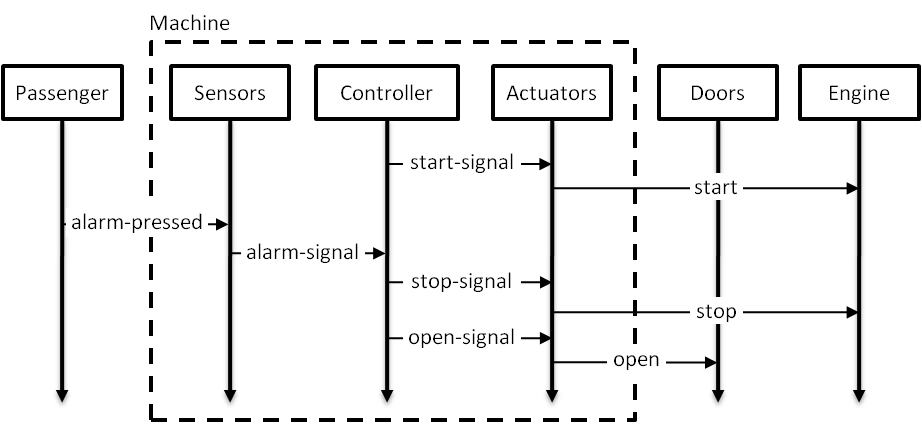
\includegraphics{src/2-framework/images/train-scenario-all-agents}
}
\caption{A scenario illustrating a train system stopping in emergency when an alarm is pressed.\label{image:train-scenario-all-agents}}
\end{figure}

\section{Agents, System and their Behavior}

A system is commonly admitted to be made of active components, called \emph{agents}, that behave and interact so as to fulfill system goals while restricting their behavior to ensure constraints they are assigned to~\cite{Feather:1987}. Some of them are human agents (the passenger), others are physical or electronic devices (e.g. the doors, the actuators), still others are software components (the automated controller). In addition to the notion of \emph{system}, being the composition of all agents, the literature often makes use of specific terms to distinguish between certain agents and/or agent aggregations. In~\cite{VanLamsweerde:2009} for example, the \emph{software-to-be} denotes the software agent(s) to be developed (the automaton controller, for example), while other agents compose its \emph{environment}. Another boundary consists in distinguishing the software together with its input and output devices from other agents. This boundary, depicted with a dashed line in Fig.\ref{image:train-scenario-all-agents}, corresponds to the distinction made by Jackson between the \emph{world} and the \emph{machine}~\cite{Jackson:1995}.

In this thesis, we are mainly interested in modeling agent \emph{behaviors}. In particular, we focus on the behavior of an agent as observed by the other agents with which it interacts (as opposed to its internal implementation). Therefore, we need specific models to capture the behavior of a single agent and operators on such models to be able to play with agent boundaries, e.g. capturing the behavior of agent aggregations like the \emph{software environment}, the \emph{machine} or simply, the \emph{system}. 

We choose to model agent behaviors and interactions in an event-based framework, where they communicate via messages that are sent and received instantaneously. Such kind of communication, called \emph{handshaking} communication, leads to a \emph{synchronous} event-based framework. This is motivated by the simplicity of this setting, an important aspect for accessibility to stakeholders involved during the early-design phase of a system. The next section introduces the kind of models used to capture agent behaviors while the next one presents operators for composing (and decomposing) them synchronously.

\subsection{Agents as Labeled Transition Systems}

In our framework, the behavior of an agent, say \artifact{Ag}, is modeled by a specific kind of finite state machine, called \emph{labeled transition system} (LTS). This formalism, initially introduced by Keller for reasoning about parallel programs~\cite{Keller:1976}, has since been intensively used for specifying and analyzing concurrent systems, e.g. in~\cite{Milner:1989, Clarke:1989, Magee:1997}. A LTS is made of a set of states and a set of transitions between them (see Fig.\ref{image:framework-start-stop}). Each transition is labeled with an \emph{event} name -- sometimes called an \emph{action} name; also, a specific state is the \emph{initial state}, designated graphically by an empty arrow in front of it (state 0 in the figure). 

\begin{figure}[H]
\centering\scalebox{0.8}{
  \includegraphics*{src/2-framework/images/start-stop}}
  \caption{A Labeled Transition System for an \artifact{Engine} agent\label{image:framework-start-stop}.}
\end{figure}

We say that a LTS \emph{transits} from a state $P_i$ to a state $P_j$ with an event $evt$, and we denote it by $P_i \stackrel{evt}{\longrightarrow} P_j$, if there is a transition labeled with that event name between those states.

The \emph{alphabet} of an agent, denoted by $\Sigma_{Ag}$ (or $\Sigma$ for short if the agent is clear),  denotes the set of event names that the agent recognizes. At first glance, therefore, the alphabet of an agent is composed of the different labels depicted on its LTS. In the example at hand, \artifact{$\Sigma_{Engine}=\{start, stop\}$}. The alphabet captures the notion of \emph{agent interface}, as a set of observable events, and naturally drives the way the agent interacts with its environment (see the notion of agent composition later).

By definition in this thesis, the \emph{behavior} of an agent is the (infinite) set of finite traces that its LTS accepts. It is also called its \emph{language} and will be noted $\mathcal{L}(Ag)$. A trace is a sequence of event names, and will be written between \verb|<| and \verb|>| brackets. Loosely speaking, a trace is accepted by a LTS if it denotes an existing path in the corresponding graph, starting in the initial state. Note that, by this definition, a prefix of an accepted trace is also an accepted trace; the empty trace $\lambda$ is therefore always accepted. For example, the LTS of Fig.\ref{image:framework-start-stop} accepts the trace \artifact{<start stop start>}, and hence \artifact{<start stop>}, but not \artifact{<start start>}. The corresponding \emph{language} is $\mathcal{L}(\artifact{Engine})=\{\lambda$, \artifact{<start>}, \artifact{<start stop>}, \artifact{<start stop start>}, \ldots $\}$

Now, if an agent and its behavior -- as traces admitted by its LTS -- are conceptually two different things, we are almost exclusively concerned here with behavioral aspects of agents. For this reason and unless the context demands making a clear distinction, we'll often use the term \emph{agent} to actually denote its LTS. Similarly, we'll often use the term \emph{alphabet} (or \emph{language}) of a LTS directly. The formal definitions given later support us in doing so.

Last, but not least, we assume \emph{deterministic} agents in this thesis, and strongly rely -- yet sometimes subtly -- on this hypothesis. This choice allows keeping our modeling framework conceptually simple to use and intuitive for stakeholders involved in the early design phase that our techniques target. From a conceptual point of view, such an assumption means that the state of an agent at a given time is uniquely determined by the sequence of events it has ``processed'' from its initial state. It also means that the agent will react to subsequent events on a pre-defined and known way, that does not depend on non-observable phenomena that happened in the past or could happen in the future (in other words, everything necessary to distinguish between two different agent states is explicitly modeled). An agent is deterministic if and only if its LTS is itself deterministic. A LTS is deterministic if no state has two outgoing transitions labeled with the same event name and does not make use of non-observable transitions -- the so-called $\tau$ transitions. Note that many authors use more complex frameworks for specifying and verifying concurrent and/or distributed systems. In particular, the related literature on process algebra does not make a deterministic assumption similar to ours, see e.g. \cite{Hoare:1985}, \cite{Milner:1989} and \cite{Magee:1999}.

This deterministic assumption has important consequences on our framework, and on the soundness of our synthesis techniques. In particular, under our assumption, two states of an LTS (resp. two LTS) may safely be considered equivalent if they accept the same set of traces (resp. they accept the same set of traces from their respective initial state), which is known as defining a \emph{trace equivalence} binary relation on LTS states (many frameworks prefer \emph{observational equivalence}~\cite{Milner:1989} as equivalence relation because it takes non-observable transitions into account for distinguishing between non-equivalent states). Our choice allows approaching the notion of agent behavior in terms of the language it accepts. In particular we can safely restrict our attention to agent behaviors defined by the class of \emph{regular} languages~\cite{Hopcroft:1979}, a necessary hypothesis for inductive behavior synthesis presented in chapter~\ref{chapter:inductive-synthesis}. Note that regular languages are also assumed by authors that rely on scenarios for modeling and/or verifying concurrent systems, see e.g.~\cite{Alur:1999, Uchitel:2003, Uchitel:2004}.

\subsection{System as Agent composition}

If a system is composed of active agents and the behavior of each of these agents is explicitly modeled with an LTS, one can ask what is the behavior of the system itself. We define it through parallel composition~\cite{Hoare:1985}, for a setting where agents execute asynchronously but synchronize on all shared event names. Given a system made of $n$ agents, and the composition operator denoted by~$\parallel$, the system is defined as:

\begin{center}
$System = Ag_1~\parallel~...~\parallel~Ag_n$ 
\end{center}

As we are interrested in agent \emph{behaviors} only, we use the binary composition operator $\parallel$ defined on LTS (the operator is both commutative and associative, allowing our writing above). This operator allows computing the interleaving of all event traces under the constraint that the two LTS must synchronize on shared event names. Let assume two agents whose LTS are $P$ and $Q$ respectively. The composition $P \parallel Q$ is another LTS whose state space is defined on the Cartesian product of the states of $P$ and $Q$. In other words a composite state $P_i \parallel Q_i$ models the fact that the first agent is in state~$P_i$ and the other in state~$Q_i$. From the interleaving semantics, in such a state, either both LTS transit on a shared event or one transits on a non-shared event while the other stays in its previous state:

\begin{eqnarray*}
\frac{P_i \stackrel{evt}{\longrightarrow} P_j,~Q_i \stackrel{evt}{\longrightarrow} Q_j}{P_i \parallel Q_i \stackrel{evt}{\longrightarrow} P_j \parallel Q_j}~~evt \in \Sigma_P \cap \Sigma_Q \\
\frac{P_i \stackrel{evt}{\longrightarrow} P_j}{P_i \parallel Q_i \stackrel{evt}{\longrightarrow} P_j \parallel Q_i}~~evt \in \Sigma_P \setminus \Sigma_Q \\
\frac{Q_i \stackrel{evt}{\longrightarrow} Q_j}{P_i \parallel Q_i \stackrel{evt}{\longrightarrow} P_i \parallel Q_j}~~evt \in \Sigma_Q \setminus \Sigma_P
\end{eqnarray*}

The resulting LTS can be computed constructively by exploring the state space from its initial state, defined as $P_0 \parallel Q_0$, following the three rules above.

If the notion of agent composition gives a sound interpretation to the notion of \emph{system}, it is, in fact, slighlty more general. 


%\begin{definition}[Labeled Transition System]
%A labeled transition system is a 4-tuple $(Q,\Sigma,\delta,q_0)$ where $Q$ is a finite set of states, $\Sigma$ is a set of event names n alphabet, $\delta$ is a transition function mapping $Q\times\Sigma$ to $2^Q$ and $q_0$ is the initial state. The LTS is said to be \emph{deterministic} if for any $q$ in Q and any $e$ in $\Sigma$, $\delta(q,e)$ has at most one member. 
%\end{definition}


